\documentclass[11pt, oneside]{article}   	% use "amsart" instead of "article" for AMSLaTeX format
\usepackage{geometry}                		% See geometry.pdf to learn the layout options. There are lots.
\geometry{letterpaper}                   		% ... or a4paper or a5paper or ... 
%\geometry{landscape}                		% Activate for for rotated page geometry
%\usepackage[parfill]{parskip}    		% Activate to begin paragraphs with an empty line rather than an indent
\usepackage{graphicx}				% Use pdf, png, jpg, or eps§ with pdflatex; use eps in DVI mode
								% TeX will automatically convert eps --> pdf in pdflatex		
\usepackage{amssymb}
\usepackage{amsmath}
\usepackage{parskip}
\usepackage{color}

\title{Gravity}
%\author{The Author}
%\section{}
% \subsection*{R code}
\date{}							% Activate to display a given date or no date

\graphicspath{{/Users/telliott_admin/Dropbox/Tex/png/}}

% \begin{center} 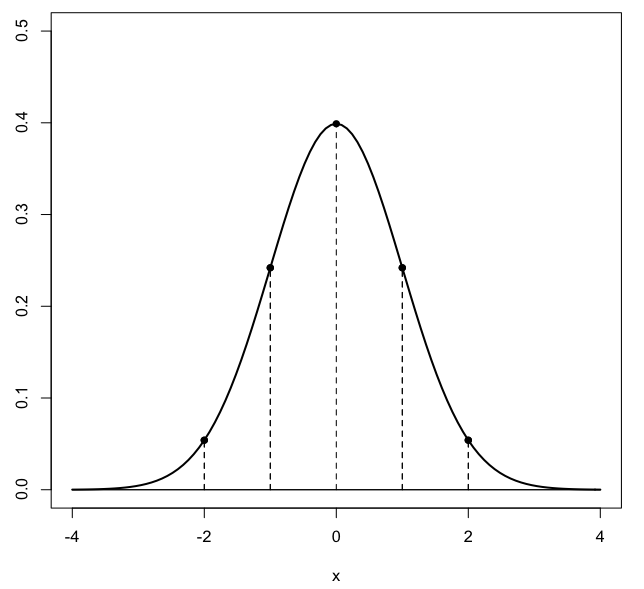
\includegraphics [scale=0.4] {gauss3.png} \end{center}

\begin{document}
\maketitle
\Large
\noindent
The simplest kind of motion is movement in a single dimension.  To analyze it, the first thing we need to do is to pick an origin for our coordinate system, the place where $x$ or $y=0$.  For a gravity problem the only dimension is up and down, and usually it's most convenient to pick the ground as the origin.  

Next, we need to decide when to start the clock, to say when is $t=0$.

Then, in physics such problems are often problems with constant acceleration due to gravity, with $\mathbf{a}=-9.8$ m/sec$^2$.  For simplicity we can take $\mathbf{a}=-10$ m/sec$^2$.  The minus sign indicates that our coordinate system assigns positive numbers to positions further above us than ground-level, while the acceleration due to gravity points toward the earth.  In 1D, we need not worry about vectors and direction, we just have to remember the convention about sign.

Velocity is the derivative of position with respect to time.
\[ v = \frac{dx}{dt} \]
and acceleration is the second derivative
\[ a = \frac{d^2x}{dt^2} = \frac{dv}{dt} \]
The two pieces of information with which we usually start the analysis are the initial position $x_0$ and the initial velocity $v_0$.  We seek an equation that will tell us the current position, $x(t)$, given these two values plus the acceleration.  Rather than do a formal integration, we make a a guess based on the relationship to the second derivative above:
\[ x(t) \approx at^2 + C \]
We need to adjust the guess to get rid of the $2$ that will come down when we take the first derivative.
\[ x(t) = \frac{1}{2}at^2 + C \]
We also realize that the constant $C$ can include two terms of two types.  First, anything like $t$ times something will go away when we take the second derivative, so we should write
\[ x(t) = \frac{1}{2}at^2 + C_1t + C_2 \]
(where $C_1$ and $C_2$ are now different constants of integration).  If we take the first derivative we have
\[ v(t) = \frac{dx}{dt} = at + C_1 \]
and we recognize that $C_1$ is just the initial velocity
\[ v(0) = v_0 = 0 + C_1 \]
so we have
\[ x(t) = \frac{1}{2}at^2 + v_0t + C_2 \]
Finally, we realize that, for $t=0$ we have
\[ x(0) = C_2 = x_0 \]
so, finally
\[ x(t) = \frac{1}{2}at^2 + v_0t + x_0 \]
which should be very familiar.  With this equation in hand, knowing $a$, $v_0$ and $t_0$, we have only two variables, $x$ and $t$.  Given $t$ it is easy to solve for $x$.  Similarly, we can solve for $v$ given $t$ using
\[ v(t) = at + v_0 \]

It can be a little awkward to find $t$ corresponding to a given $x$, but the last equation provides a nice trick for this.  Solve for $t$ (simplify the notation by using $v(t) = v$):
\[ v-v_0 = at \]
\[ t = \frac{v - v_0}{a} \]
Now, given $v$ (for example $v=0$ at the top of the curve) we can find $t$.  We can also plug this into the other equation and get something simple and useful.  Rather than write $x(t)$ just write $x$ so
\[ x = \frac{1}{2}at^2 + v_0t + x_0 \]
\[ 2(x-x_0) = at^2 + 2v_0t \]
\[ 2(x-x_0) = a \ (\frac{v - v_0}{a})^2 + 2v_0 \ (\frac{v - v_0}{a}) \ \]
\[ 2a(x - x_0) = (v - v_0)^2 + 2 v_0 (v - v_0) \ \]
\[ = v^2 - 2v v_0 + v_0^2 + 2v_0 v - 2v_0^2  \]
\[ = v^2  - v_0^2  \]
So finally,
\[ 2a(x - x_0) = v^2  - v_0^2  \]
\[ v^2 = v_0^2 + 2a(x - x_0) \]
Rather than find the time first and plug into the standard equation to get the velocity, we can go directly between velocity and position or vice versa.

Here are our equations re-written for gravity problems:
\[ y(t) = -\frac{1}{2}gt^2 + v_0t + y_0 \]
\[ v - v_0 = -gt \]
\[ v^2 = v_0^2 - 2g(y - y_0) \]
\subsection*{general examples}
One simple question is:  what is the time to fall from a given height $h$.  The initial velocity is zero, so
\[ y(t) = -\frac{1}{2}gt^2 + v_0t + y_0 \]
\[ y - y_0 = 0 - h = -h = -\frac{1}{2}gt^2 \]
\[ t = \sqrt{\frac{2h}{g}} \]
And given this time, the terminal velocity is:
\[ v = v_0 - gt = 0 - g \sqrt{\frac{2h}{g}} = -\sqrt{2gh} \]
The second simple situation is to fire a projectile up with initial velocity $u$.  Then we ask, what is the maximum height.  This is one way
\[ v^2 = v_0^2 - 2g(y - y_0) \]
\[ 0 = u^2 - 2gh \]
\[ h = \frac{u^2}{2g} \]
Another way is to first get the time:
\[ v - v_0 = -gt \]
\[ - u = -gt \]
\[ t = \frac{u}{g} \]
Now the height is
\[ y(t) = -\frac{1}{2}gt^2 + v_0t + y_0 \]
\[ h = -\frac{1}{2}g(\frac{u}{g})^2 + u\frac{u}{g} \]
\[ h = \frac{u^2}{2g}  \]
The object returns to earth when the height is equal to zero
\[ 0 = -\frac{1}{2}gt^2 + ut \]
\[ u = \frac{1}{2}gt \]
\[ t = \frac{2u}{g} \]
One-half the time is spent going up, and the other half coming down.  It's worth pointing out that the change in potential energy at height $h$ is equal to 
\[ U = mgh = mg \frac{u^2}{2g} = \frac{1}{2} m u^2 \]
which is equal to the kinetic energy at launch.

\subsection*{clever derivation}
Shankar offers this derivation in his first Physics lecture.  Write
\[ \frac{dv}{dt} = a \]
Multiply both sides by $v$
\[ v \frac{dv}{dt} = av \]
The first key step is to recognize that the left-hand side is equal (by the chain rule) to 
\[ v \frac{dv}{dt} = \frac{d}{dt} (\frac{v^2}{2}) \]
So rewrite what we had including this and on the right-hand side use the definition $v = dx/dt$
\[ \frac{d}{dt} (\frac{v^2}{2}) = a \ \frac{dx}{dt} \]
The second key is to recognize that we can get rid of $dt$ and just think about this as an equality between differentials
\[ d(\frac{v^2}{2}) = a \ dx \]
Now integrate
\[ \int d(\frac{v^2}{2}) = \int a \ dx \]
for the constants of integration use the initial values
\[ \frac{v^2}{2} - \frac{v_0^2}{2} = a (x - x_0) \]
That should look familiar:
\[ v^2 = v_0^2 + 2a (x - x_0) \]

\subsection*{numerical examples}
Suppose you are on the roof of a building of height $y_0=15$ m and throw a rock upward with velocity $v_0=10$ m/s.  We find the maximum height as the position where $v=0$.  From the second equation
\[ t = \frac{v-v_0}{a} = \frac{0 - 10}{-10} = 1 \ \text{s} \]
\[ y = \frac{1}{2}at^2 + v_0t + y_0 =  (-5) t^2 + (10) t + 15 = 20 \ \text{m} \]
How fast is it going when it hits the ground?  From the third equation
\[ v^2 = v_0^2 + 2a(y - y_0) = (10)^2 + 2(-10)(-15) = 400 \]
\[ v = \sqrt{v^2} = \sqrt{400} = \pm \ 20 \ \text{m/s} \]
There are two solutions, the one with negative value corresponds to the rock hitting the ground at the end of the throw.  The positive velocity is the same rock being thrown from the ground upward with velocity $20$ m/s.  This will also hit the ground with velocity $-20$ m/s.  

To find the time when the rock hits the ground, from the first equation
\[ y(t) = \frac{1}{2}at^2 + v_0t + y_0 = 0 = (-5)t^2 + 10t + 15 \]
\[ t^2 - 2t - 3 = 0 = (t-3)(t+1) = 0 \]
So either $t = 3$ or $t = -1$ seconds.  The first solution is the one we thought we wanted, the second corresponds to the positive velocity situation we had above.  For a throw from the ground up, the trajectory is symmetric, two seconds going up and two seconds coming back down again.  And reusing the second equation, for the part coming down $v - v_0 = at$, so  $v = at = -20$ m/s.

\end{document}  